\mytitle{Tipos de radiações}    
\addchaptersummary{Tipos de radiações}{Sumario/Figs_Sumario/FigArtigo3.jpg}{Entenda o que é radiação, como se classificam e conheça algumas de suas aplicações, bem como a importância dos materiais de blindagem de radiação!}{Murilo Aparecido da Silva} 
\newcommand{\artigotres}{\begin{center}\textcolor{base}{\MakeUppercase{Tipos de radiações}}\end{center}}

\mytitlesubtitle{e a importância de materiais para blindagem contra radiação}  

\begin{multicols}{2}

\mysubtitle{Primeiros Contatos}

A história da radiação teve seu início com as descobertas de Wilhelm K. Röntgen (Figura \ref{fig:RontgenBecquerel}), em 1895. Em suas pesquisas sobre a propagação de raios catódicos, ele havia produzido radiação eletromagnética no comprimento de onda dos raios X. Tal feito possibilitou a outros cientistas o início de mais pesquisas sobre radiações, como é o caso de Henri Becquerel (Figura \ref{fig:RontgenBecquerel}), que estudou as características de substâncias fosforescentes e fluorescentes, além das propriedades de sais de urânio que o levaram à descoberta da radioatividade.

\begin{figure}[H]
			\centering
			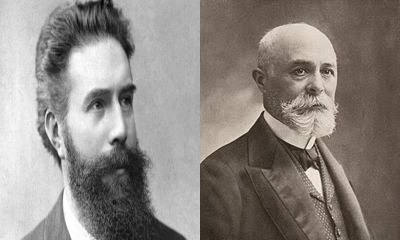
\includegraphics[width=\linewidth]{Figuras/Artigo3/Rontgen_e_Becquerel.png}
			\caption{Wilhelm K. Röntgen (à esquerda) [Fonte: \href{https://www3.unicentro.br/petfisica/2018/03/02/wilhelm-conrad-rontgen-1845-1923/}{Unicentro Pet Física}] e Henri Becquerel (à direita) [Fonte: \href{https://www3.unicentro.br/petfisica/2017/06/22/antoine-henri-becquerel-1852-1908/}{Unicentro Pet Física}].}
			\label{fig:RontgenBecquerel}
\end{figure}

Procedendo os trabalhos iniciados por Becquerel, o casal Marie e Pierre Curie (Figura \ref{fig:MarieEPierre}) descobriu outros dois elementos químicos que também eram capazes de emitir radiação:  Rádio (Ra) e Polônio (Po) \refdois{ref1:artigo3}{ref2:artigo3}.

\mysubtitle{O que é radiação? Como se classificam? Quais suas aplicações?}

Radiações são ondas eletromagnéticas ou partículas que se propagam com uma determinada velocidade. Possuem energia e cargas elétrica e magnética, podendo ser geradas por fontes naturais ou por dispositivos construídos pelo homem. Elas apresentam energia variável desde valores pequenos até muito elevados \reftres{ref1:artigo3}{ref2:artigo3}{ref7:artigo3}.

\begin{figure}[H]
			\centering
			
\includegraphics[width=\linewidth]{Figuras/Artigo3/Marie & Pierre Curie.png}
			\caption{Marie e Pierre Curie. [Fonte: \href{https://brasilescola.uol.com.br/quimica/maria-curie-descoberta-radioatividade.htm}{Brasil Escola}].}
			\label{fig:MarieEPierre}
\end{figure}


As radiações eletromagnéticas mais conhecidas são: luz, micro-ondas, ondas de rádio, radar, laser, raios X e gama. As radiações sob a forma de partículas – com massa, carga elétrica e carga magnética – mais comuns são os feixes de elétrons, os feixes de prótons, a radiação beta e a radiação alfa \ref{ref7:artigo3}.

Devido ao seu amplo intervalo energético, uma radiação pode ser descrita como não ionizante ou ionizante a depender de sua energia, o termo ionização dá nome ao processo pelo qual um átomo ou molécula adquire carga negativa ou positiva ao ganhar ou perder elétrons, esse processo pode se dar por meio da colisão entre partículas como ilustra a Figura \ref{fig:ProcessoIonizacao}. 



	
As \textit{radiações não ionizantes}, por exemplo, possuem consideravelmente baixa energia e baixa frequência, obedecendo assim a Lei de Planck $E=h\nu$, sendo o tipo de radiação mais presente em nosso dia a dia. Alguns casos particulares são o calor, ondas de rádio e a luz, todas formas de radiação não ionizante. Sem este tipo de radiação não poderíamos apreciar um programa de TV em nossas casas ou cozinhar em um forno micro-ondas \refdois{ref1:artigo3}{ref2:artigo3}.

\begin{figure}[H]
			\centering
			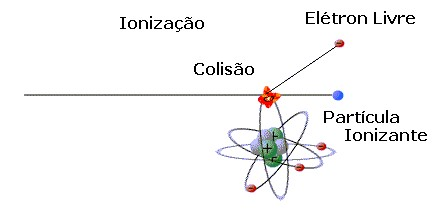
\includegraphics[width=0.9\linewidth]{Figuras/Artigo3/ionização.jpg}
			\caption{Diagrama esquemático do processo de ionização. [Fonte: \href{https://www.fisica.net/aplicada/biofisica/radiacao.php}{física.net}].}
			\label{fig:ProcessoIonizacao}
\end{figure}



Já as \textit{radiações ionizantes} são um tipo de radiação menos presente em nosso cotidiano habitual: é um tipo de radiação que possui altos níveis de energia e altas frequências quando comparadas às radiações não ionizantes. De forma geral, as radiações ionizantes são aquelas que têm energia suficiente para provocar ionização em átomos e moléculas, tornando eletricamente carregado o meio físico em que penetra. Seus efeitos podem ser danosos para as células, afetando o material genético e causando doenças graves, como o câncer. Alguns tipos de radiação ionizante são as partículas alfa e beta, os raios gama e os raios-X \ref{ref1:artigo3}. 



\end{multicols}

\begin{figure}[H]
            \centering
			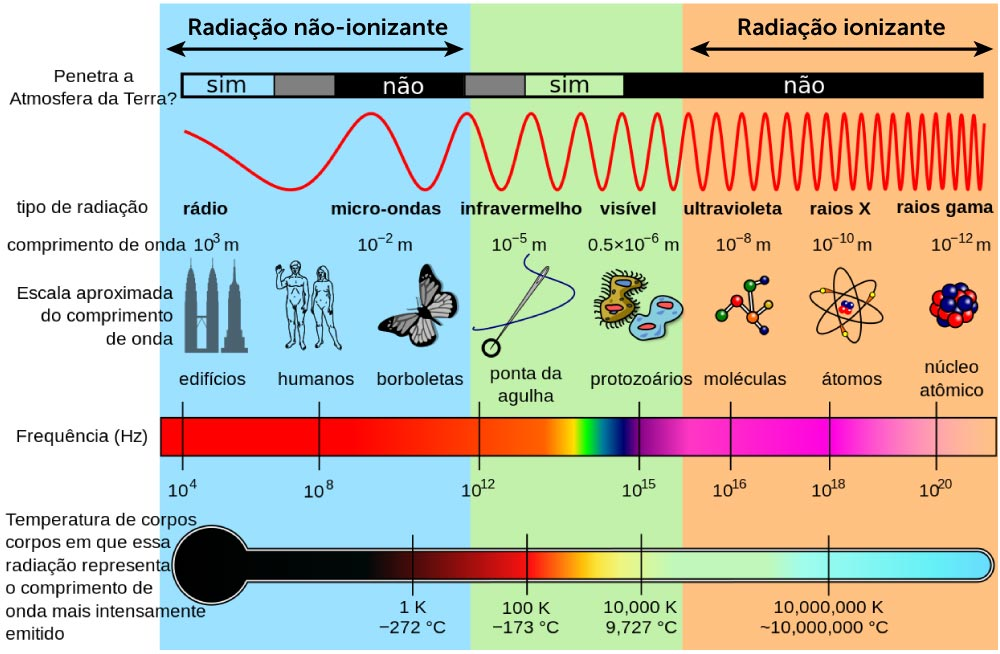
\includegraphics[width=0.9\linewidth]{Figuras/Artigo3/radiacao.jpg}
			\caption{Diagrama esquemático dos tipos de radiações. [Fonte: \href{https://www.sapralandauer.com.br/protecao-radiologica-saiba-sobre-os-principais-aspectos-normas-e-tecnologias-empregadas/o-que-e-radiacao-nocoes-basicas-de-protecao-radiologica/\#toggle-id-2}{Sapralandauer}].}
			\label{fig:DiagramaEsq}
\end{figure}

\begin{multicols}{2}

Suas principais aplicações se dão nas área de saúde - em radiografias, tomografias, exames de densitometria óssea, entre outros - e alimentícia (...), matando micro-organismos presentes em frutas, verduras e legumes, fazendo com que durem mais tempo e sejam mais saudáveis para o consumo \ref{ref8:artigo3}.

Na Figura \ref{fig:DiagramaEsq}, está um diagrama esquemático dos tipos de radiação, sua frequência, e uma escala aproximada de seu comprimento de onda.

\mysubtitle{Materiais para blindagem contra radiação ionizante}

Devido ao perigo que as radiações ionizantes podem nos oferecer, ao longo das décadas diferentes materiais para proteção contra elas foram produzidos a fim de proteger os seres humanos e seus arredores de seu impacto destrutivo \ref{ref8:artigo3}.

Os materiais utilizados para tal finalidade devem possuir alta densidade a fim de se alcançar uma forte habilidade de blindagem. Por esse motivo, são comumente usados materiais como o chumbo e o concreto.

Entretanto, materiais livres de chumbo têm ganhado nos últimos anos notória apreciação por parte dos pesquisadores, pois o chumbo é um material tóxico. Assim muitas pesquisas visam propor novos materiais que não possuem toxicidade como meio de blindagem. 

Em especial, pode-se citar os vidros livres de chumbo, que, por possuírem boa transparência à luz visível e, mais importante ainda, sua composição, espessura e densidade pode ser alterada e controlada durante o processo de preparação. Isso os credencia como um material promissor para o desenvolvimento de diferentes tipos de equipamentos de proteção contra radiação, como protetores faciais e janelas de salas de raios X \ref{ref9:artigo3}.

Tendo em vista tudo que foi apresentado, temos, mesmo que de forma sucinta, a percepção do que é radiação e a importância de seu uso e aplicações em nosso mundo. Também entendemos a importância dos materiais utilizados em proteção radiológica, pois a radiação ionizante, mesmo sendo tão benéfica nos mais diversos meios, ainda pode nos ser prejudicial à saúde. Por isso, temos que ter em vista a importância de seu uso controlado e a utilização de equipamentos que visem a nossa proteção quando necessário seu uso. Vimos também a importância da pesquisa de materiais que não sejam tóxicos, buscando assim por novas substâncias que não sejam prejudiciais à nossa saúde.

\authorinfo{Murilo Aparecido}{http://lattes.cnpq.br/2055729643800351}




\end{multicols}